\let\negmedspace\undefined
\let\negthickspace\undefined
\documentclass[journal]{IEEEtran}
\usepackage[a5paper, margin=10mm, onecolumn]{geometry}
%\usepackage{lmodern} % Ensure lmodern is loaded for pdflatex
\usepackage{tfrupee} % Include tfrupee package

\setlength{\headheight}{1cm} % Set the height of the header box
\setlength{\headsep}{0mm}     % Set the distance between the header box and the top of the text

\usepackage{gvv-book}
\usepackage{gvv}
\usepackage{cite}
\usepackage{amsmath,amssymb,amsfonts,amsthm}
\usepackage{algorithmic}
\usepackage{graphicx}
\usepackage{textcomp}
\usepackage{xcolor}
\usepackage{txfonts}
\usepackage{listings}
\usepackage{enumitem}
\usepackage{mathtools}
\usepackage{gensymb}
\usepackage{comment}
\usepackage[breaklinks=true]{hyperref}
\usepackage{tkz-euclide} 
\usepackage{listings}
% \usepackage{gvv}                                        
\def\inputGnumericTable{}                                 
\usepackage[latin1]{inputenc}                                
\usepackage{color}                                            
\usepackage{array}                                            
\usepackage{longtable}                                       
\usepackage{calc}                                             
\usepackage{multirow}                                         
\usepackage{hhline}                                           
\usepackage{ifthen}                                           
\usepackage{lscape}
\begin{document}
\bibliographystyle{IEEEtran}
\vspace{3cm}

\title{JEE MAINS 2024\\April 8 - Shift 1}
\author{EE24BTECH11061 - Rohith Sai}
\maketitle

\renewcommand{\thefigure}{\theenumi}
\renewcommand{\thetable}{\theenumi}

\section*{Integer Type}
\begin{enumerate}
\item Let the area of the region enclosed by the curve $y=min\{\sin{x}, \cos{x}\}$ and the x-axis between $x=-\pi$ and $x=\pi$ be $A$. Then $A^2$ is equal to

\item The number of 3-digit numbers, formed using the digits 2, 3, 4, 5 and 7, when the repetition of digits is not allowed, and which are not divisible by 3, is equal to

\item Let $\vec{a} = 9i-13j+25k$, $\vec{b} = 3i+7j-13k$ and $\vec{c} = 17i-2j+k$ be three given vectors. If $\vec{r}$ is a vector such that $\vec{r}\times\vec{a} = \brak{\vec{b} + \vec{c}}\times\vec{a}$ and $\vec{r}\cdot\brak{\vec{b} - \vec{c}} = 0$, then $\frac{\abs{593\vec{r}+67\vec{a}}^2}{\brak{593}^2}$ is equal to

\item If the range of $f\brak{\theta} = \frac{\sin^4{\theta}+3\cos^2{\theta}}{\sin^4{\theta}+\cos^2{\theta}}$, $\theta \in \mathbb{R}$ is $\sbrak{\alpha,\beta}$, then the sum of the infinite G.P., whose first term is 64 and the common ratio is $\frac{\alpha}{\beta}$, is equal to

\item Let $A = \myvec{2 & -1\\1 & 1}$. If the sum of diagonal elements of $A^{13}$ is $3^n$, then $n$ is equal to

\item Let $\alpha = \sum^n_{r=0} \brak{4r^2+2r+1} ^nC_r$ and $\beta = \brak{\sum^n_{r=0} \frac{^nC_r}{r+1}} + \frac{1}{n+1}$. If $140 < \frac{22\alpha}{\beta}<281$, then the value of $n$ is

\item The value of $\lim_{x \to 0} 2\brak{\frac{1-\cos{x}\sqrt{\cos{2x}}\sqrt[3]{\cos{3x}}\dots\dots\sqrt[10]{\cos{10x}}}{x^2}}$ is

\item Three balls are drawn at random from a bag containing 5 blue and 4 yellow balls. Let the random variables $X$ and $Y$ respectively denote the number of blue and yellow balls. If $\overline{X}$ and $\overline{Y}$ are the means of $X$ and $Y$ respectively, then $7\overline{X} + 4\overline{Y}$ is equal to

\item If the orthocentre of the triangle formed by the lines $2x+3y-1 = 0$, $x+2y-1 = 0$ and $ax + by - 1=0$, is the centroid of another triangle, whose circumcentre and orthocentre respectively are $\brak{3,4}$ and $\brak{-6,-8}$, then the value of $\abs{a-b}$ is

\item Let the positive integers be written in the form:
\begin{figure}[htp]
    \centering
    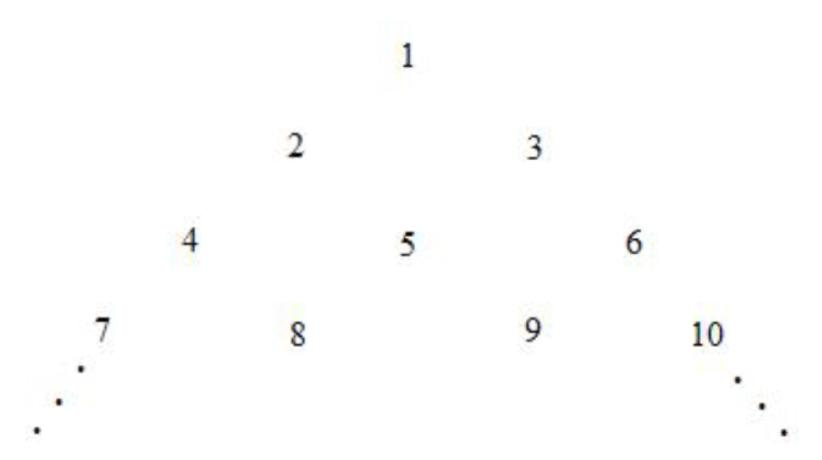
\includegraphics[width=6cm]{figs/figure.png}
    \label{fig:figure}
\end{figure}\\
If the $k^{th}$ row contains exactly $k$ numbers for every natural number $k$, then the row in which the number 5310 will be, is

\end{enumerate}
\end{document}